\documentclass[12pt,compress,english,utf8,t]{beamer}

\usepackage{etex}

\usepackage[ngerman]{babel}

\usepackage{multicol}
\usepackage{ragged2e}
\usepackage{mathtools}
\usepackage[cmtip,all]{xy}
\newcommand{\longsquiggly}{\xymatrix{{}\ar@{~>}[r]&{}}}

\usepackage[protrusion=true,expansion=true]{microtype}

\title{Das Geheimnis der Zahl 5}
\author[Tagesabschluss des Tübinger Linuxtags]{Ingo Blechschmidt \\[0.1em] \tiny \texttt{ingo.blechschmidt@math.uni-augsburg.de}}
\institute{$(n+2)$-ter Tübinger Linuxtag}
\date{11. Juni 2016}

\usetheme{Warsaw}
\usecolortheme{seahorse}
\definecolor{mypurple}{RGB}{150,0,255}
\setbeamercolor{structure}{fg=mypurple}
\usefonttheme{serif}
\usepackage[T1]{fontenc}
\usepackage{libertine}
\useinnertheme{rectangles}
\setbeamercovered{invisible}

\setbeamertemplate{title page}[default][colsep=-1bp,rounded=false,shadow=false]
\setbeamertemplate{frametitle}[default][colsep=-2bp,rounded=false,shadow=false,center]

\setbeamertemplate{navigation symbols}{}
\setbeamertemplate{headline}{}

\newcommand*\oldmacro{}%
\let\oldmacro\insertshorttitle%
\renewcommand*\insertshorttitle{%
  \oldmacro\hfill\insertframenumber\,/\,\inserttotalframenumber\hfill}

\newcommand{\backupstart}{
  \newcounter{framenumberpreappendix}
  \setcounter{framenumberpreappendix}{\value{framenumber}}
}
\newcommand{\backupend}{
  \addtocounter{framenumberpreappendix}{-\value{framenumber}}
  \addtocounter{framenumber}{\value{framenumberpreappendix}} 
}

\newcommand{\defeq}{\vcentcolon=}

\newcommand{\hil}[1]{{\usebeamercolor[fg]{item}{\textbf{#1}}}}

\newcommand{\icfrac}[4]{#1 + \dfrac{1}{#2 + \dfrac{1}{#3 + \dfrac{1}{#4 + \ddots}}}}
\newcommand{\icfracc}[3]{\dfrac{1}{#1 + \dfrac{1}{#2 + \dfrac{1}{#3 + \ddots}}}}
\newcommand{\icfraccc}[2]{\dfrac{1}{#1 + \dfrac{1}{#2 + \ddots}}}
\newcommand{\icfracccc}[5]{#1 + \dfrac{1}{#2 + \dfrac{1}{#3 + \dfrac{1}{#4 + \dfrac{1}{#5 + \ddots}}}}}

\setbeameroption{show notes}
\setbeamertemplate{note page}[plain]

\begin{document}

\frame{
  \titlepage

  \vspace*{-2em}
  \begin{center}
    \small
    \emph{Gewidmet an Prof. Dr. Jost-Hinrich Eschenburg.}
    \medskip

    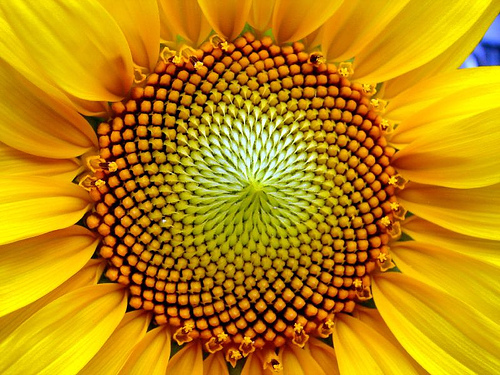
\includegraphics[height=0.25\textheight]{sonnenblume}\quad
    
\includegraphics[height=0.25\textheight]{mandelbrot}\quad
    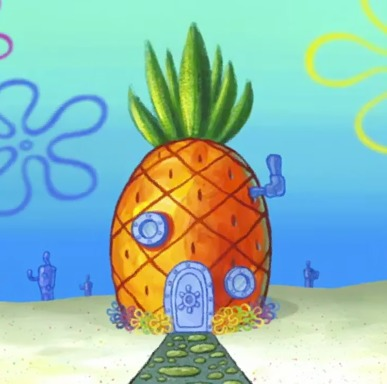
\includegraphics[height=0.25\textheight]{spongebob-ananas}
  \end{center}
}

\begin{frame}\frametitle{Gliederung}\tableofcontents\end{frame}


\section{Ein Entwurfsmuster der Natur}

\begin{frame}\frametitle{Ein Entwurfsmuster der Natur}
  \begin{center}
    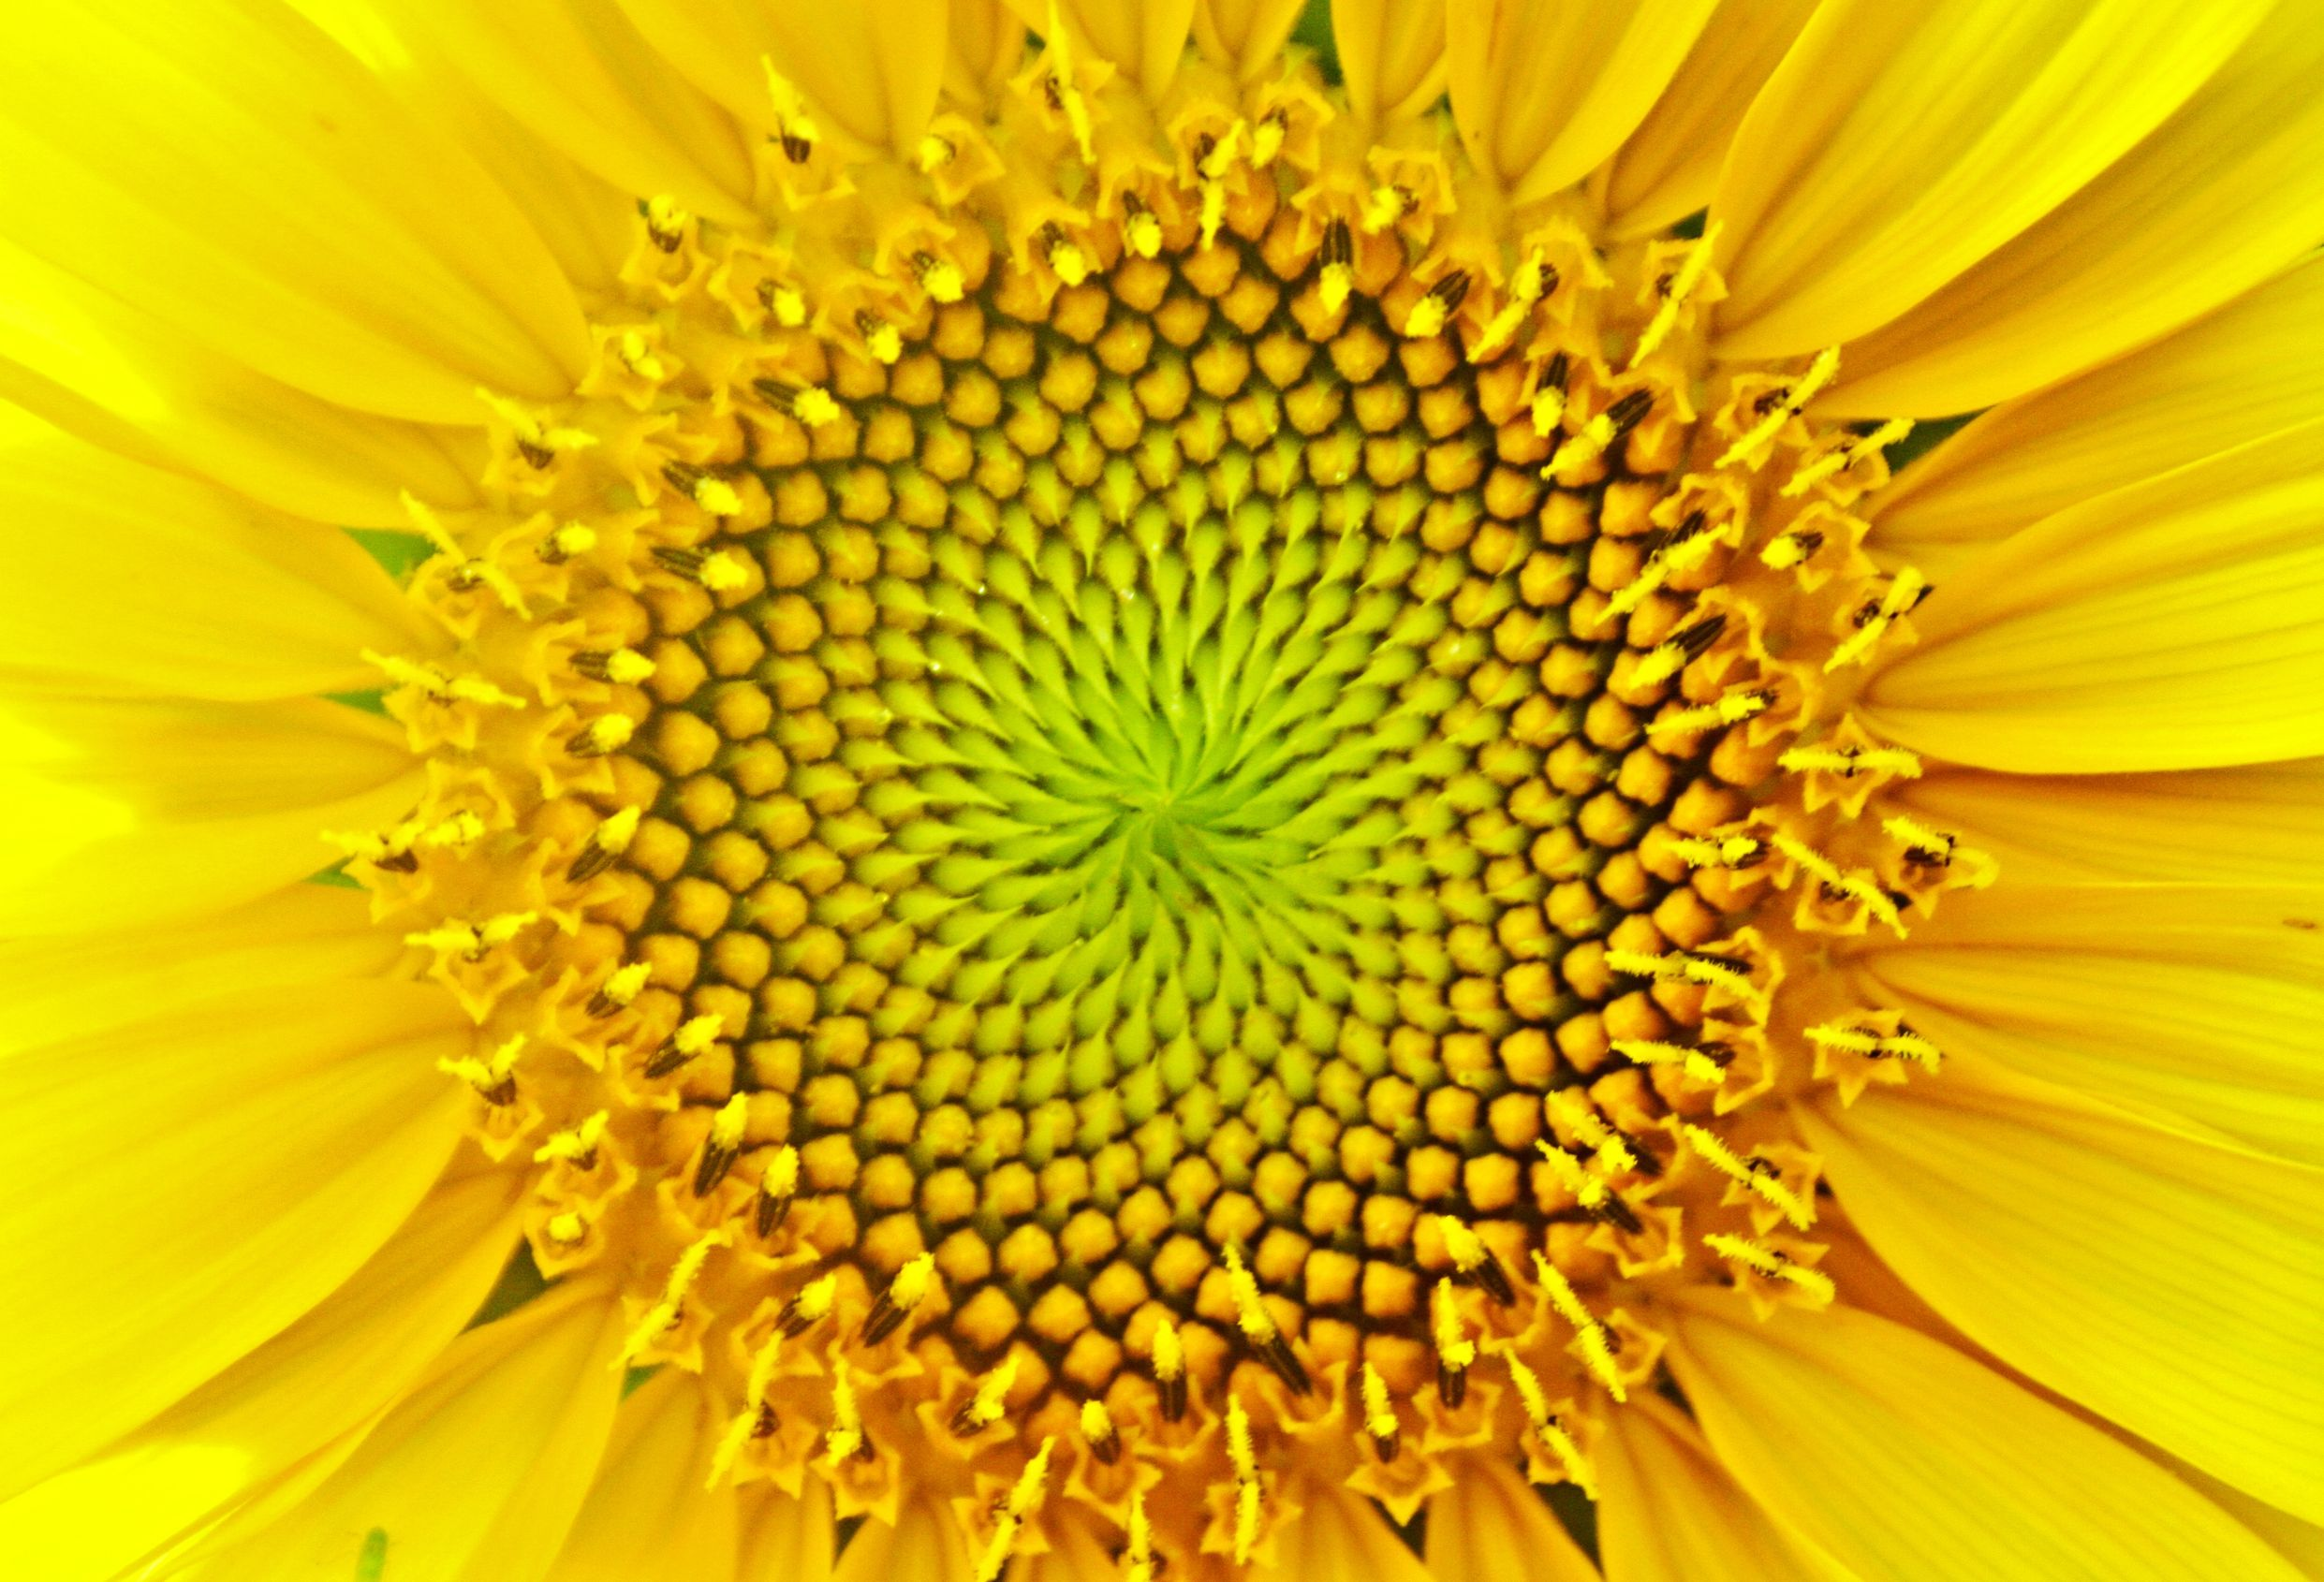
\includegraphics[height=0.6\textheight]{sonnenblume2}
    \bigskip
    % 34 counterclockwise, 21 clockwise

    \only<1>{
      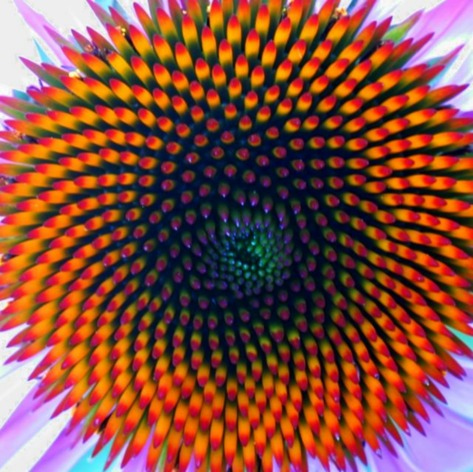
\includegraphics[height=0.2\textheight]{coneflower}\qquad
      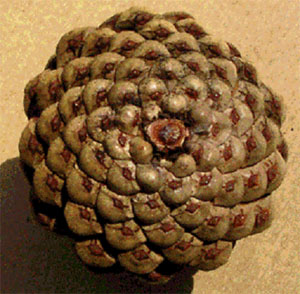
\includegraphics[height=0.2\textheight]{zapfen}\qquad
      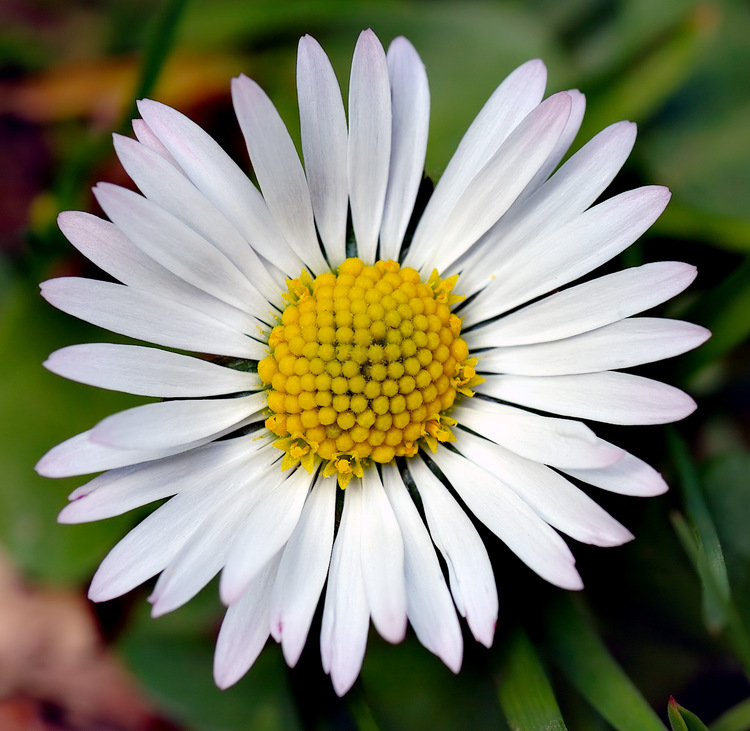
\includegraphics[height=0.2\textheight]{Bellis_perennis_white_(aka)}
    }
    \only<2>{
      \hil{Fibonaccizahlen:} \\
      1, 1, 2, 3, 5, 8, 13, 21, 34, 55, \ldots
    }
  \end{center}
\end{frame}

\note{\justifying
  Die Anzahl Spiralen auf einer Sonnenblume ist stets eine Fibonaccizahl (oder
  eine Zahl, die sehr nah an einer Fibonaccizahl ist). Etwa waren im Foto auf
  der vorherigen Folie 21 Spiralen im Uhrzeigersinn und 34 Spiralen im
  Gegenuhrzeigersinn sichtbar. Wieso bloß?
  \par
}


\section{Kettenbrüche}

\subsection{Beispiele}

\begin{frame}\frametitle{Ein merkwürdiger Bruch}
  \only<2-3>{\vspace*{-1em}}
  \only<1>{\Huge}
  \only<1-3>{\[
    \icfrac{1}{2}{2}{2} = {?}
  \]}
  \only<2-3>{\vspace*{1em}}

  \pause
  Entscheidende Beobachtung: Wenn wir
  \only<1-3>{\[ x \defeq {?} - 1 = \icfracc{2}{2}{2} \]}
  \only<4->{\[ x \defeq {?} - 1 = \icfraccc{2}{2} \]}
  \pause
  setzen, gilt
  \[ \frac{1}{2 + x} = x. \]
  \pause
  \pause

  Multiplizieren mit dem Nenner liefert
  \only<5>{$1 = x \cdot (2 + x),$}%
  \only<6->{$1 = 2x + x^2,$}
  \pause
  \pause
  also müssen wir nur die quadratische Gleichung
  $0 = x^2 + 2x - 1$
  lösen,
  \pause
  somit
  \[ x = \frac{-2 + \sqrt{8}}{2} = -1 + \sqrt{2}
    \quad\text{oder}\quad
     x = \frac{-2 - \sqrt{8}}{2} = -1 - \sqrt{2}. \]
  Es ist die positive Möglichkeit.
\end{frame}

\begin{frame}\frametitle{Weitere Beispiele}
  \only<1-2>{\vspace*{-2em}\begin{align*}
    \visible<2>{[1; 2, 2, 2, \ldots] =} \icfrac{1}{2}{2}{2} &= \sqrt{2} \\[1.5em]
    \visible<2>{[2; 4, 4, 4, \ldots] =} \icfrac{2}{4}{4}{4} &= \sqrt{5} \\[1.5em]
    \visible<2>{[3; 6, 6, 6, \ldots] =} \icfrac{3}{6}{6}{6} &= \sqrt{10}
  \end{align*}}

  \pause
  \pause

  \begin{enumerate}
    \item $\phantom{0}\sqrt{2} = [1; 2, 2, 2, 2, 2, 2, 2, 2, \ldots]$
    \item $\phantom{0}\sqrt{5} = [2; 4, 4, 4, 4, 4, 4, 4, 4, \ldots]$
    \item $\sqrt{10}           = [3; 6, 6, 6, 6, 6, 6, 6, 6, \ldots]$
    \item $\phantom{0}\sqrt{6} = [2; 2, 4, 2, 4, 2, 4, 2, 4, \ldots]$
    \item $\sqrt{14}           = [3; 1, 2, 1, 6, 1, 2, 1, 6, \ldots]$
    \item $\sbox0{$\sqrt{10}$}\makebox[\wd0][r]{$e$} = [2; 1, 2, 1, 1, 4, 1, 1, 6, \ldots]$ \\[0.2em]
    $\phantom{\sqrt{10}} = 2{,}71828182845904523536\ldots$
  \end{enumerate}
\end{frame}

\note{\justifying
  Die Ziffern der Zahl~$e = 2{,}7182818284\ldots$, der Basis des natürlichen
  Logarithmus, bilden kein erkennbares Muster. Aber die Kettenbruchentwicklung
  ist völlig regelmäßig (und das kann man auch beweisen).\par
}


\subsection{Berechnung der Kettenbruchentwicklung}

\begin{frame}\frametitle{Der euklidische Algorithmus}
  Zur Erinnerung: $\sqrt{2} = 1 + \icfracc{2}{2}{2} = 1{,}41421356\ldots$
  \bigskip

  \begin{align*}
    1{,}41421356\ldots &= 1 \cdot 1{,}00000000\ldots + 0{,}41421356\ldots \\
    1{,}00000000\ldots &= 2 \cdot 0{,}41421356\ldots + 0{,}17157287\ldots \\
    0{,}41421356\ldots &= 2 \cdot 0{,}17157287\ldots + 0{,}07106781\ldots \\
    0{,}17157287\ldots &= 2 \cdot 0{,}07106781\ldots + 0{,}02943725\ldots \\
    0{,}07106781\ldots &= 2 \cdot 0{,}02943725\ldots + 0{,}01219330\ldots \\
    0{,}02943725\ldots &= 2 \cdot 0{,}01219330\ldots + 0{,}00505063\ldots \\
    &\,\,\,\vdots
  \end{align*}
\end{frame}

\note{\justifying
  Die Rechnung auf der vorherigen Folie setzt voraus, dass man die Ziffern
  von~$\sqrt{2}$ schon hinreichend genau kennt. Aber auch, wenn das nicht der
  Fall ist, kann man den euklidischen Algorithmus verwenden. Lediglich die
  Darstellung wird komplizierter -- man rechnet dann mit lauter Termen, in
  denen~$\sqrt{2}$ vorkommt.
  \medskip

  Es gibt sogar eine geometrische Möglichkeit, um einzusehen, dass der jeweils
  kleinere Rest immer zweimal in den jeweils größeren Rest passt.
  \par
}

\note{\justifying
  Wieso liefert der euklidische Algorithmus die Koeffizienten der
  Kettenbruchentwicklung? Um das einzusehen, schreiben wir
  \begin{align*}
    x   &= a_0 \cdot \sbox0{$r_0$}\makebox[\wd0][l]{$1$} + r_0 \\
    1   &= a_1 \cdot r_0 + r_1 \\
    r_0 &= a_2 \cdot r_1 + r_2 \\
    r_1 &= a_3 \cdot r_2 + r_3
  \end{align*}
  und so weiter. Dabei sind die Zahlen~$a_n$ natürliche Zahlen und die Reste~$r_n$
  sind jeweils kleiner als der zweite Faktor des jeweiligen nebenstehenden
  Produkts. Dann gilt:
  \begin{align*}
    x &= a_0 + r_0 = a_0 + 1/(1/r_0) \\
      &= a_0 + 1/(a_1 + r_1/r_0) = a_0 + 1/(a_1 + 1/(r_0/r_1)) \\
      &= a_0 + 1/(a_1 + 1/(a_2 + r_2/r_1)) = \cdots
  \end{align*}
}

\note{\justifying
  In der wunderschönen Programmiersprache Haskell ist der Code, um die
  unendliche Kettenbruchentwicklung zu berechnen, nur eine Zeile lang (die
  Typdeklaration ist optional):
  \medskip

  {\scriptsize\texttt{cf :: Double -> [Integer]}\\
  \texttt{cf x = a : cf (1 / (x - fromIntegral a)) where a = floor x}\par}
  \medskip

  Die Kettenbruchentwicklung einer Zahl~$x$ beginnt also mit~$a$, dem
  ganzzahligen Anteil von~$x$, und geht dann mit der Kettenbruchentwicklung
  von~$1 / (x-a)$ weiter.
  \medskip

  Wegen Rundungsfehlern kann man sich nur auf die ersten paar Terme
  der Entwicklung verlassen. Zum Beispiel könnte~\texttt{cf (sqrt 6)} folgendes
  Ergebnis liefern:
  \[ \texttt{[2,2,4,2,4,2,4,2,4,2,4,2,4,2,4,2,2,1,48,2,4,6,1,\ldots\!\!]}. \]
  \par
}


\subsection{Bestapproximationen durch die Kettenbruchentwicklung}

\begin{frame}\frametitle{Bestapproximationen durch Kettenbrüche}
  \begin{theorem}
  Wenn man die Kettenbruchentwicklung einer Zahl~$x$ abschneidet, erhält man
  einen Bruch~$a/b$, der unter allen Brüchen mit Nenner~$\leq b$ der Zahl~$x$
  am nächsten liegt.
  \end{theorem}
  \[
    \sqrt{2} = \icfrac{1}{2}{2}{2} \longsquiggly
    1 + \dfrac{1}{2 + \dfrac{1}{2 + \dfrac{1}{2}}} = \frac{17}{12} \approx 1{,}42
  \]
  \medskip
  \pause

  \hil{Bonus.} Je größer der Koeffizient nach der Abschneidestelle ist, desto
  besser ist die Näherung~$a/b$.
\end{frame}

\note{\justifying
  Präziser formuliert besagt der Zusatz, dass die Entfernung von~$x$ zu~$a/b$
  kleiner als~$1 / (a_n a_{n+1})$ ist, wobei~$a_n$ der letzte Koeffizient
  unmittelbar vor der Abschneidestelle und~$a_{n+1}$ der erste Koeffizient
  direkt danach ist.
  \par
}


\section{\texorpdfstring{Approximationen von $\pi$}{Approximationen von π}}

\begin{frame}[plain,c]
  \centering\Huge
  \scalebox{2.8}{\hil{Liebe ist}} \\[0.6em]
  \scalebox{2.8}{\hil{wichtig.}}

  \bigskip
  \bigskip

  \scalebox{2.8}{\hil{$\boldsymbol{\heartsuit}$}}
  \par
\end{frame}

\begin{frame}[plain,c]
  \centering\Huge
  \scalebox{2.8}{\hil{Pi ist}} \\[0.6em]
  \scalebox{2.8}{\hil{wichtig.}}

  \bigskip
  \bigskip

  \scalebox{2.8}{\hil{$\boldsymbol{\pi}$}}
  \par
\end{frame}

\begin{frame}\frametitle{Approximationen von $\pi$}
  \[ \pi = 3{,}1415926535\ldots = \icfracccc{3}{7}{15}{1}{292} \]

  \begin{enumerate}
    \item $3$
    \item $[3;7]\phantom{,15,1} = \phantom{0}22/7\phantom{00} = \underline{3{,}14}28571428\ldots$
    \item $[3;7,15]\phantom{,1} = 333/106 = \underline{3{,}1415}094339\ldots$
    \item $[3;7,15,1] = 355/113 = \underline{3{,}141592}9203\ldots$ (Milü)
  \end{enumerate}
\end{frame}

\note{\justifying
  Man weiß natürlich nicht mit Sicherheit, wie in der Antike Näherungen
  für~$\pi$ berechnet wurden. Vorstellbar ist aber, dass eine Form des
  euklidischen Algorithmus eingesetzt wurde (natürlich nicht mit Dezimalbrüchen
  notiert, sondern zum Beispiel mit Schnüren unterschiedlicher Längen
  durchgeführt).
  \medskip

  Weil der Koeffizient~$292$ in der Kettenbruchentwicklung von~$\pi$
  exzeptionell groß ist, ist die Approximation~$355/113$ exzeptionell gut.
  Das ist ein schöner mathematischer Zufall! Mir gefällt die Vorstellung, dass
  bessere Approximationen in der Antike nicht berechenbar waren, aber dass dank
  dieses Zufalls die beste noch zugängliche Approximation tatsächlich eine
  außerordentlich gute war. Insbesondere ist sie viel besser, als der
  Nenner~$113$ vermuten lassen würde.
  \medskip

  NB: Die Näherung~$355/113$ kann man sich leicht einprägen (11--33--55).
  % XXX: NB
  \par
}


\section{Das Mandelbrot-Fraktal}

\begin{frame}\frametitle{Das Mandelbrot-Fraktal}
  \centering
  
\includegraphics[width=0.8\textwidth]{mandelbrot}
  \medskip
  \pause

  Im Mandelbrot-Fraktal tauchen die Fibonaccizahlen auf.
  \par
\end{frame}

\note{\justifying
  Eine Erklärung, wo und weshalb die Fibonaccizahlen im Mandelbrot-Fraktal
  auftreten, steht auf \url{http://math.bu.edu/DYSYS/FRACGEOM2/node7.html}.\par
}


\section{Spiralen in der Natur}

\begin{frame}\frametitle{Spiralen in der Natur}
  \centering
  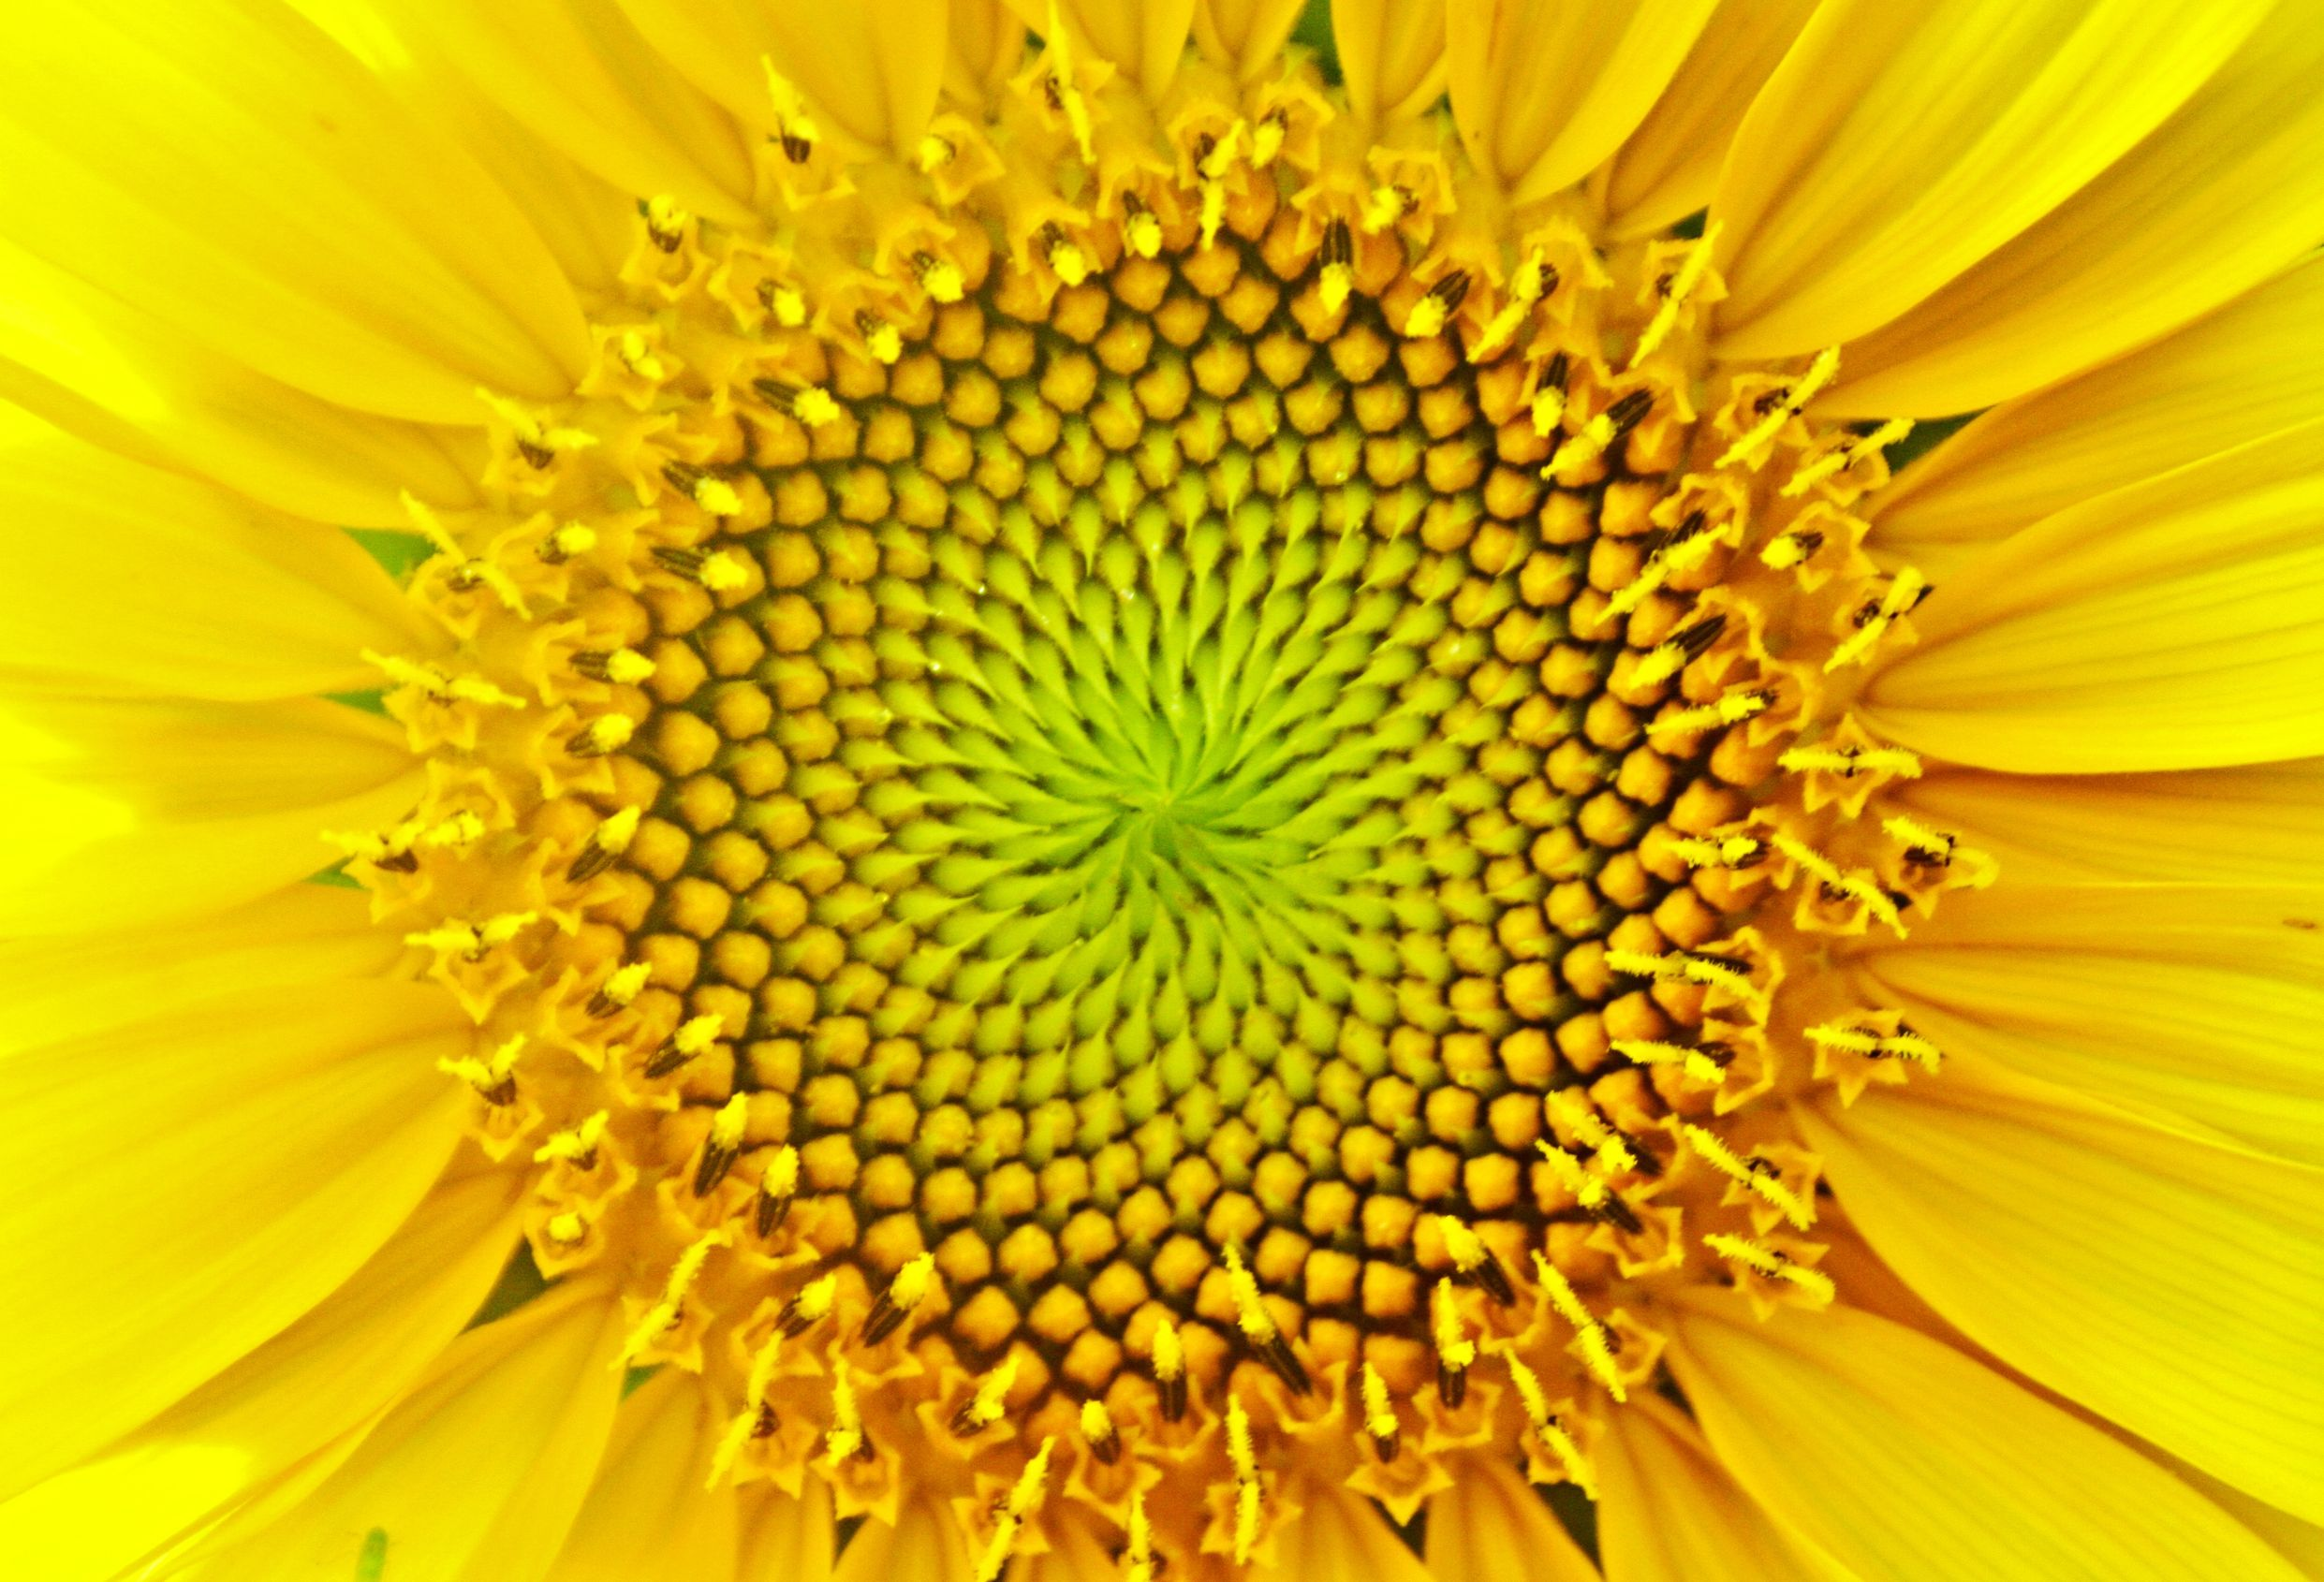
\includegraphics[height=0.8\textheight]{sonnenblume2}
  \par
\end{frame}

\begin{frame}\frametitle{Die irrationalste aller Zahlen}
  \small
  Der optimale Winkel für aufeinanderfolgende Samen ist weder
  \[ 90^\circ = \frac{1}{4} \cdot 360^\circ \qquad\text{noch}\qquad
    45^\circ = \frac{1}{8} \cdot 360^\circ. \]
  \pause
  Stattdessen ist er der \hil{goldene Winkel} $\Phi \cdot 360^\circ \approx
  582^\circ$ (äqv.: $138^\circ$):

  \begin{center}
    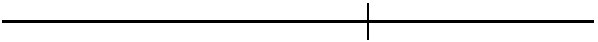
\includegraphics[width=0.7\textwidth]{golden-ratio}
  \end{center}
  \[ \Phi = \text{\hil{goldener Schnitt}} = \frac{1 + \sqrt{5}}{2} = 1{,}6180339887\ldots \]

  \begin{theorem}Der goldene Schnitt~$\Phi$ ist die \hil{irrationalste aller
  Zahlen}.\end{theorem}
  \pause
  \medskip
  \textbf{Beweis.} $\Phi = \icfrac{1}{1}{1}{1}.$
\end{frame}

\note{\justifying
  Der goldene Schnitt kommt an vielen Stellen in Natur und Kunst vor.
  Wenn man eine Strecke im goldenen Schnitt teilt, so wird das längere
  Teilstück genau~$\Phi$ mal so groß sein wie das kleinere Teilstück.
  Konzeptioneller:
  {\footnotesize\[\text{Gesamtstrecke} : \text{längeres Teilstück} =
    \text{längeres Teilstück} : \text{kürzeres Teilstück}. \]\par}

  Wenn man einen Bruchanteil~$\frac{a}{b}$ des Vollkreises als Drehwinkel
  verwendet, ist man nach~$b$ Umdrehungen wieder am Ausgangsort angelangt.
  Das ist schlecht! So vergeudet man Platz.
  \medskip

  Es ist besser, einen Anteil des Vollkreises zu nehmen, der \emph{nicht} als
  Bruchzahl ausgedrückt werden kann -- eine \emph{irrationale Zahl}. Von allen
  irrationalen Zahlen sollte man die wählen, die \emph{am irrationalsten} ist.
  \medskip

  Eine Zahl lässt sich umso besser durch Brüche approximieren, je größer die
  Koeffizienten in der Kettenbruchentwicklung sind. Bei~$\Phi$ sind die
  Koeffizienten dagegen so klein wie nur möglich. Das ist der Grund,
  wieso~$\Phi$ die "`irrationalste"' Zahl ist. Sie ist von allen Zahlen die,
  die sich am schwersten durch Brüche annähern lässt.\par
  % XXX umso
}

\begin{frame}\frametitle{(Nicht-)Verwendung des goldenen Winkels}
  \centering
  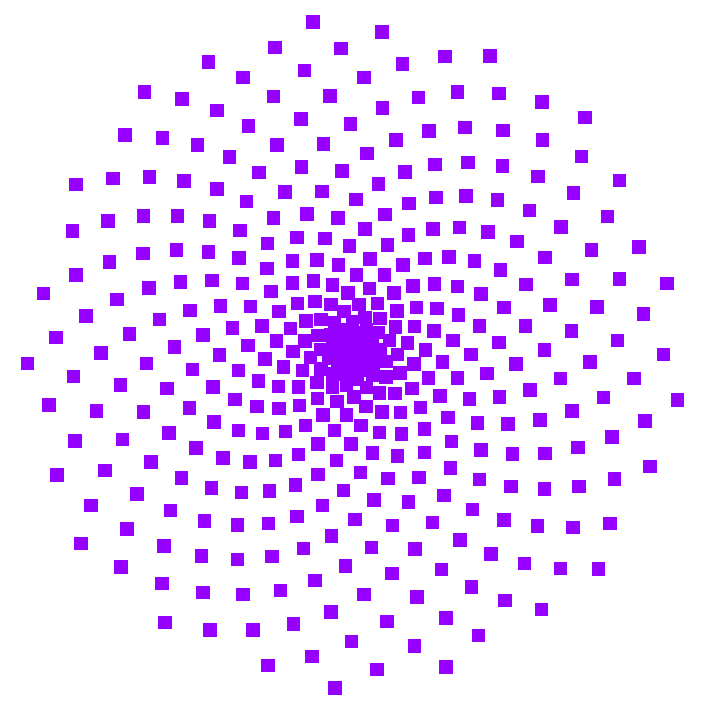
\includegraphics[width=0.45\textwidth]{drehwinkel-400-1_61803398874989484820.pdf}

  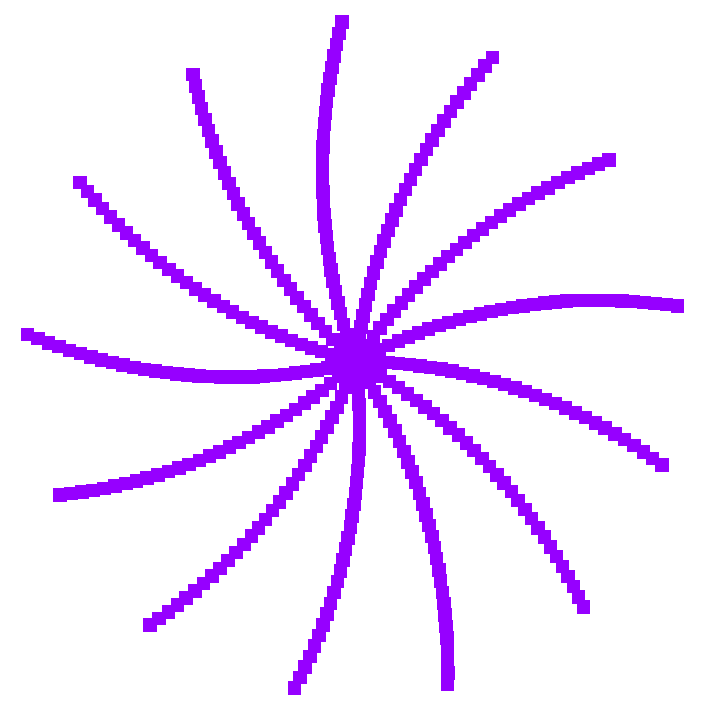
\includegraphics[width=0.25\textwidth]{drehwinkel-400-1_61525621097211707043.pdf}
  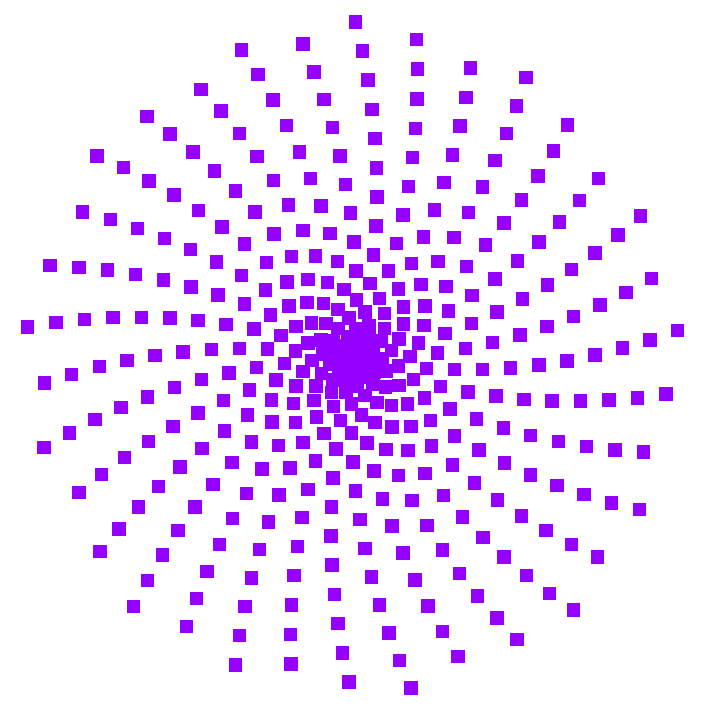
\includegraphics[width=0.25\textwidth]{drehwinkel-400-1_61775621097211707043.pdf}
  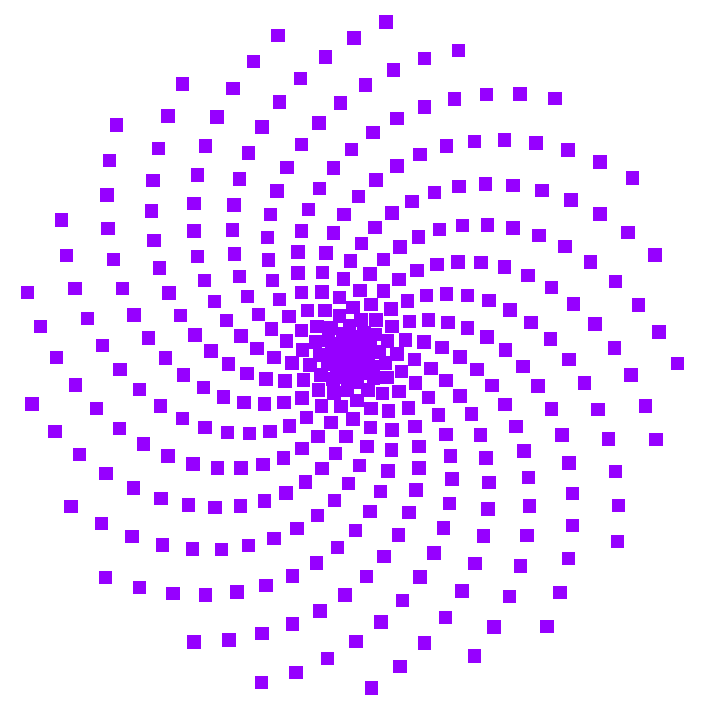
\includegraphics[width=0.25\textwidth]{drehwinkel-400-1_61831176652767262597.pdf}
  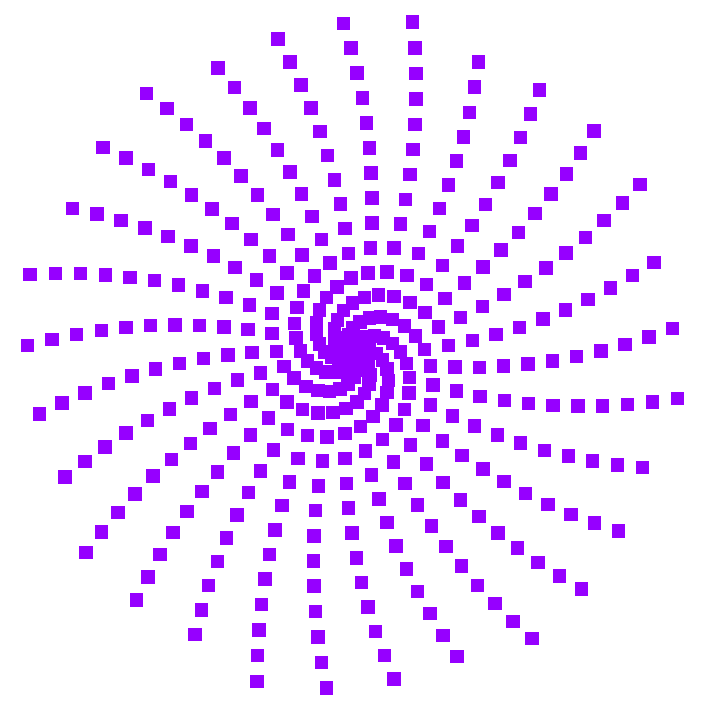
\includegraphics[width=0.25\textwidth]{drehwinkel-400-1_62081176652767262597.pdf}
  \par
\end{frame}

\note{\justifying
  In der oberen Abbildung wurde der goldene Winkel verwendet. Die Winkel in den
  anderen vier Abbildungen waren dagegen:
  \begin{enumerate}
    \item $\text{goldener Winkel} - 1^\circ$
    \item $\text{goldener Winkel} - 0{,}1^\circ$
    \item $\text{goldener Winkel} + 0{,}1^\circ$
    \item $\text{goldener Winkel} + 1^\circ$
  \end{enumerate}

  Der Code, der diese Abbildungen erzeugt hat, ist online unter
  \url{https://github.com/iblech/number5}. Probiere doch deine
  Lieblingszahlen als Drehwinkel aus!
  \medskip

  Du bist herzlich eingeladen, eine tolle interaktive JavaScript/Canvas-Demo zu
  schreiben. Verwende die folgenden einfachen Formeln, um bei einem
  Drehwinkel~$\varphi$ die Koordinaten des~$n$-ten Punkts zu berechnen
  (die Einheiten sind so, dass $\varphi = 1/4$ den Winkel $90^\circ$ bedeutet).
  \begin{align*}
    x &= n \cdot \cos(2 \pi \varphi \cdot n) \\
    y &= n \cdot \sin(2 \pi \varphi \cdot n)
  \end{align*}
}

\note{\centering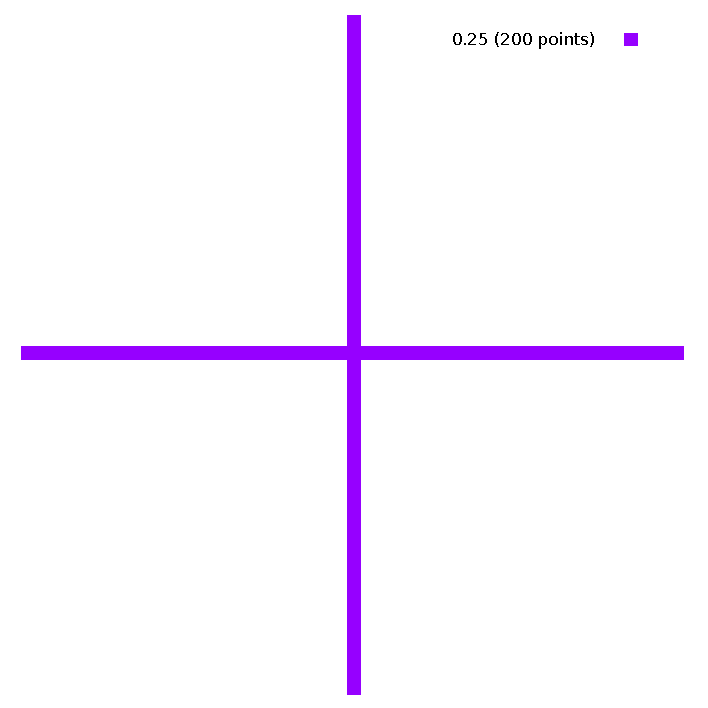
\includegraphics[height=0.95\textheight]{drehwinkel-200-0_25.pdf}\par}
\note{\centering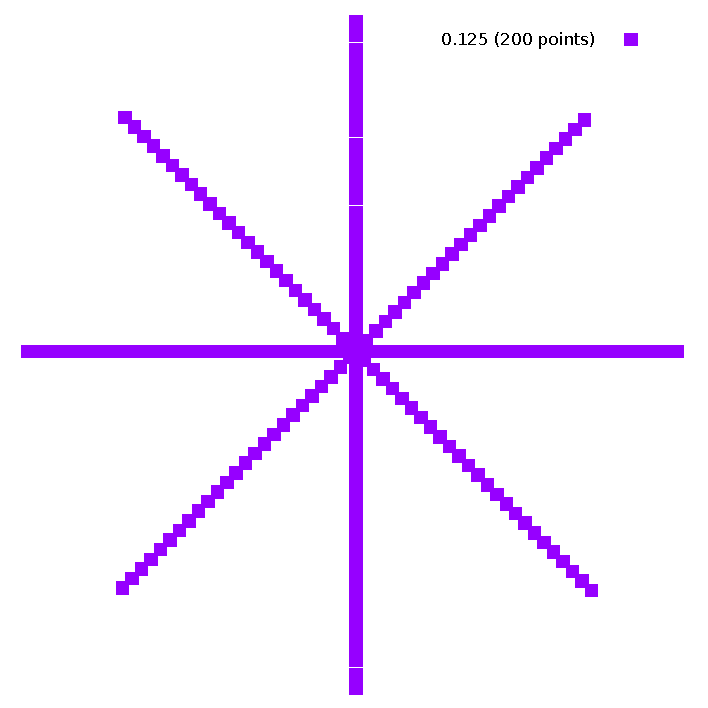
\includegraphics[height=0.95\textheight]{drehwinkel-200-0_125.pdf}\par}
\note{\centering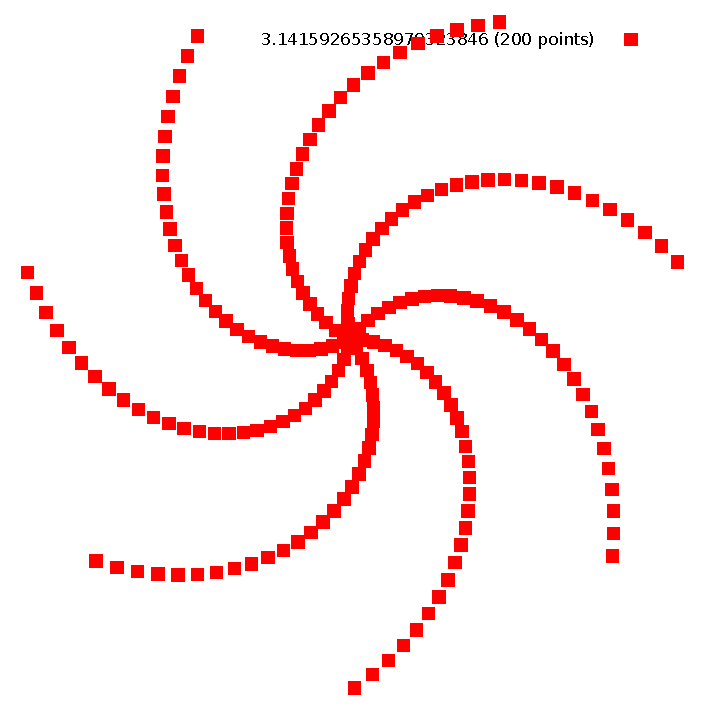
\includegraphics[height=0.95\textheight]{drehwinkel-200-3_14159265358979323846.pdf}\par}
\note{\centering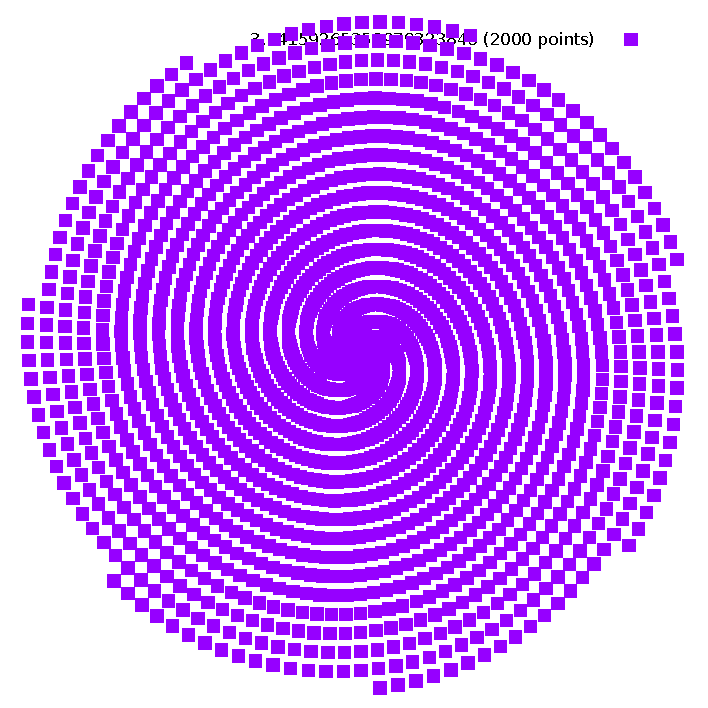
\includegraphics[height=0.95\textheight]{drehwinkel-2000-3_14159265358979323846.pdf}\par}
\note{\centering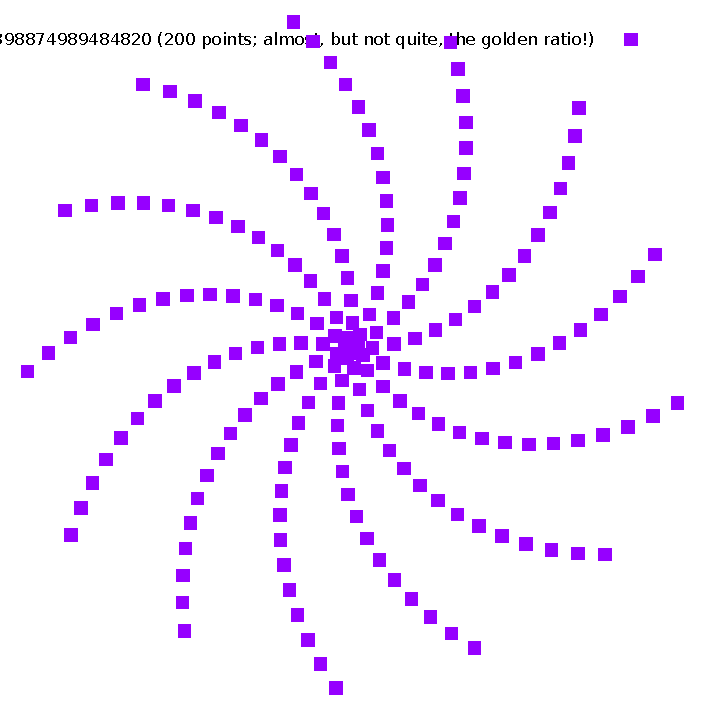
\includegraphics[height=0.95\textheight]{drehwinkel-200-1_61603398874989484820.pdf}\par}
\note{\centering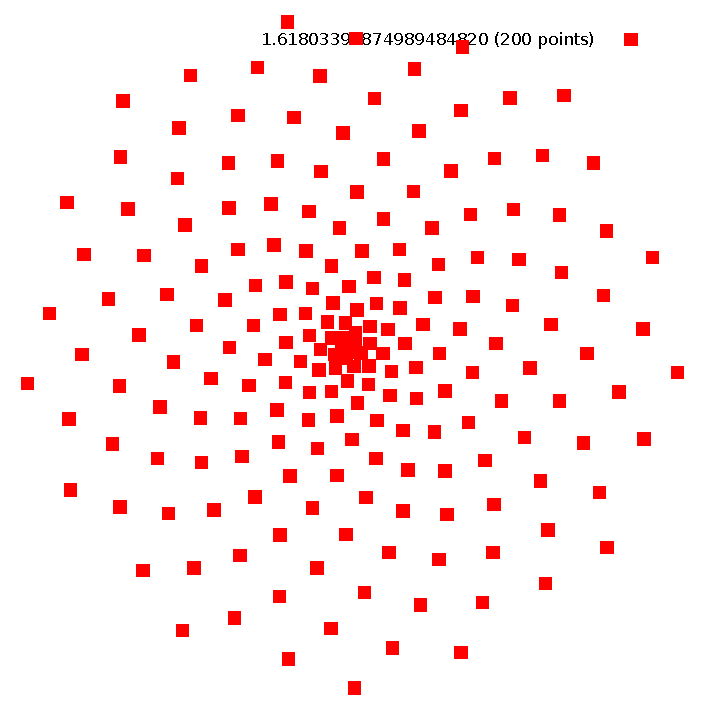
\includegraphics[height=0.95\textheight]{drehwinkel-200-1_61803398874989484820.pdf}\par}
\note{\centering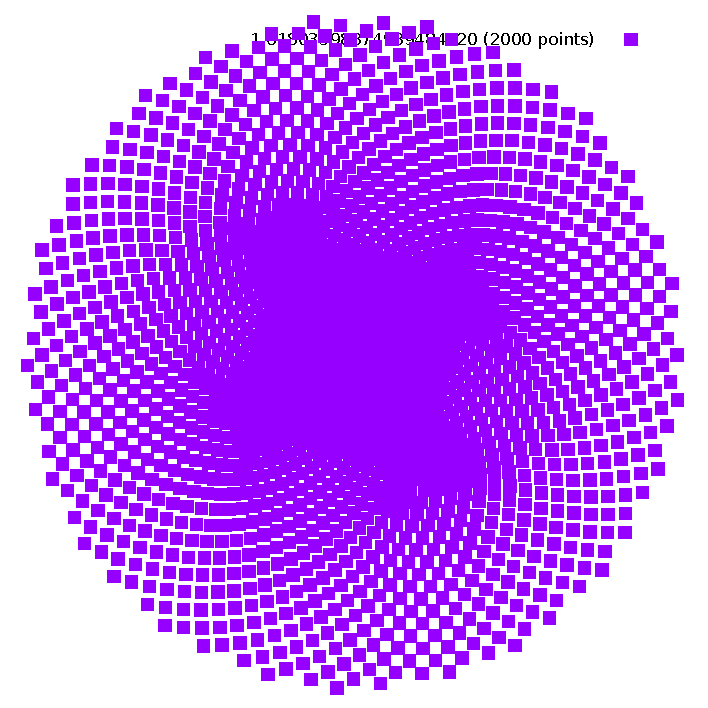
\includegraphics[height=0.95\textheight]{drehwinkel-2000-1_61803398874989484820.pdf}\par}

\begin{frame}\frametitle{Wieso die Fibonaccizahlen?}
  \vspace*{-1em}
  \[ \Phi = \icfrac{1}{1}{1}{1} \]

  \begin{enumerate}
    \item $1\phantom{[,1,1,1,1,1,1,1,1]} = \phantom{0}1/1$
    \item $[1;1]\phantom{,1,1,1,1,1,1,1} = \phantom{0}2/1$
    \item $[1;1,1]\phantom{,1,1,1,1,1,1} \pause = \phantom{0}3/2$
    \item $[1;1,1,1]\phantom{,1,1,1,1,1} \pause = \phantom{0}5/3$
    \item $[1;1,1,1,1]\phantom{,1,1,1,1} \pause = \phantom{0}8/5$ \pause
    \item $[1;1,1,1,1,1]\phantom{,1,1,1} = 13/8$
    \item $[1;1,1,1,1,1,1]\phantom{,1,1} = 21/13$
    \item $[1;1,1,1,1,1,1,1]\phantom{,1} = 34/21$
    \item $[1;1,1,1,1,1,1,1,1] = 55/34$
  \end{enumerate}
\end{frame}

\note{\justifying
  Wählt man als Drehwinkel den Anteil~$\frac{a}{b}$ des Vollkreises
  (vollständig gekürzt), so erhält man exakt~$b$ Spiralen.
  Die Animation auf
  \[ \text{\scriptsize\url{http://rawgit.com/iblech/number5/master/drehwinkel-0_3027522935779816.mp4}} \]
  zeigt einen Zoom bei Verwendung von~$33/109 \cdot 360^\circ$ als Drehwinkel.
  Die Kettenbruchentwicklung ist
  \[ \frac{33}{109} = \dfrac{1}{3 + \dfrac{1}{3 + \dfrac{1}{3 +
  \dfrac{1}{3}}}} \]
  \vspace*{-1.5em}

  mit Abschneidungen
  \[ \dfrac{1}{3}, \qquad
  \dfrac{1}{3 + \dfrac{1}{3}} = \dfrac{3}{10}, \qquad
  \dfrac{1}{3 + \dfrac{1}{3 + \dfrac{1}{3}}} = \dfrac{10}{33}.
  \]
  Daher sieht man zunächst drei, dann zehn, dann 33 und schließlich 109
  Spiralen.
}


\section{Die Ananas aus SpongeBob Schwammkopf}

\begin{frame}\frametitle{Die Ananas aus SpongeBob Schwammkopf}
  \centering
  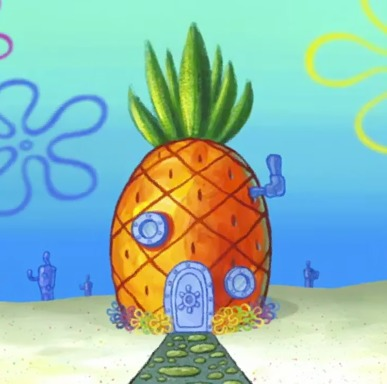
\includegraphics[width=0.65\textwidth]{spongebob-ananas}
  \medskip

  Von Vi Hart, Mathemusikerin.
  \par
\end{frame}

\note{\justifying
  Vi Hart hat ein Video mit dem Titel
  \emph{Open Letter to Nickelodeon, Re: SpongeBob's Pineapple under the Sea}
  auf YouTube: \url{https://www.youtube.com/watch?v=gBxeju8dMho}\par

  \centering
  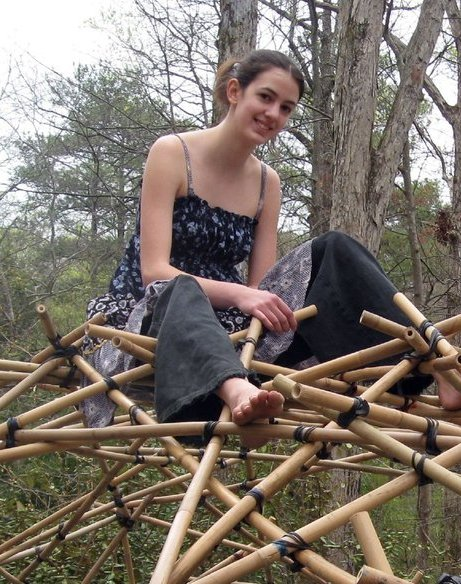
\includegraphics[width=0.3\textwidth]{vi-hart}
  \bigskip

  \emph{Lust auf Übungsaufgaben zum Thema?} \\[0.2em]
  \scriptsize
  \url{http://rawgit.com/iblech/number5/master/pizzaseminar-de.pdf}%
  \\
  Aufgabe 12 erklärt die Verbindung zwischen dem goldenen Schnitt und der Zahl~5.
  \bigskip

  \scalebox{2.8}{\large\hil{$\boldsymbol{\heartsuit}$}}
  \par
}

\appendix

\backupstart

\begin{frame}\frametitle{Mathecamp in den Ferien \\[-0.4em] \scriptsize vom 20. bis 26. August 2016 in Violau}
  \vspace{-0.4cm}
  \begin{center}
    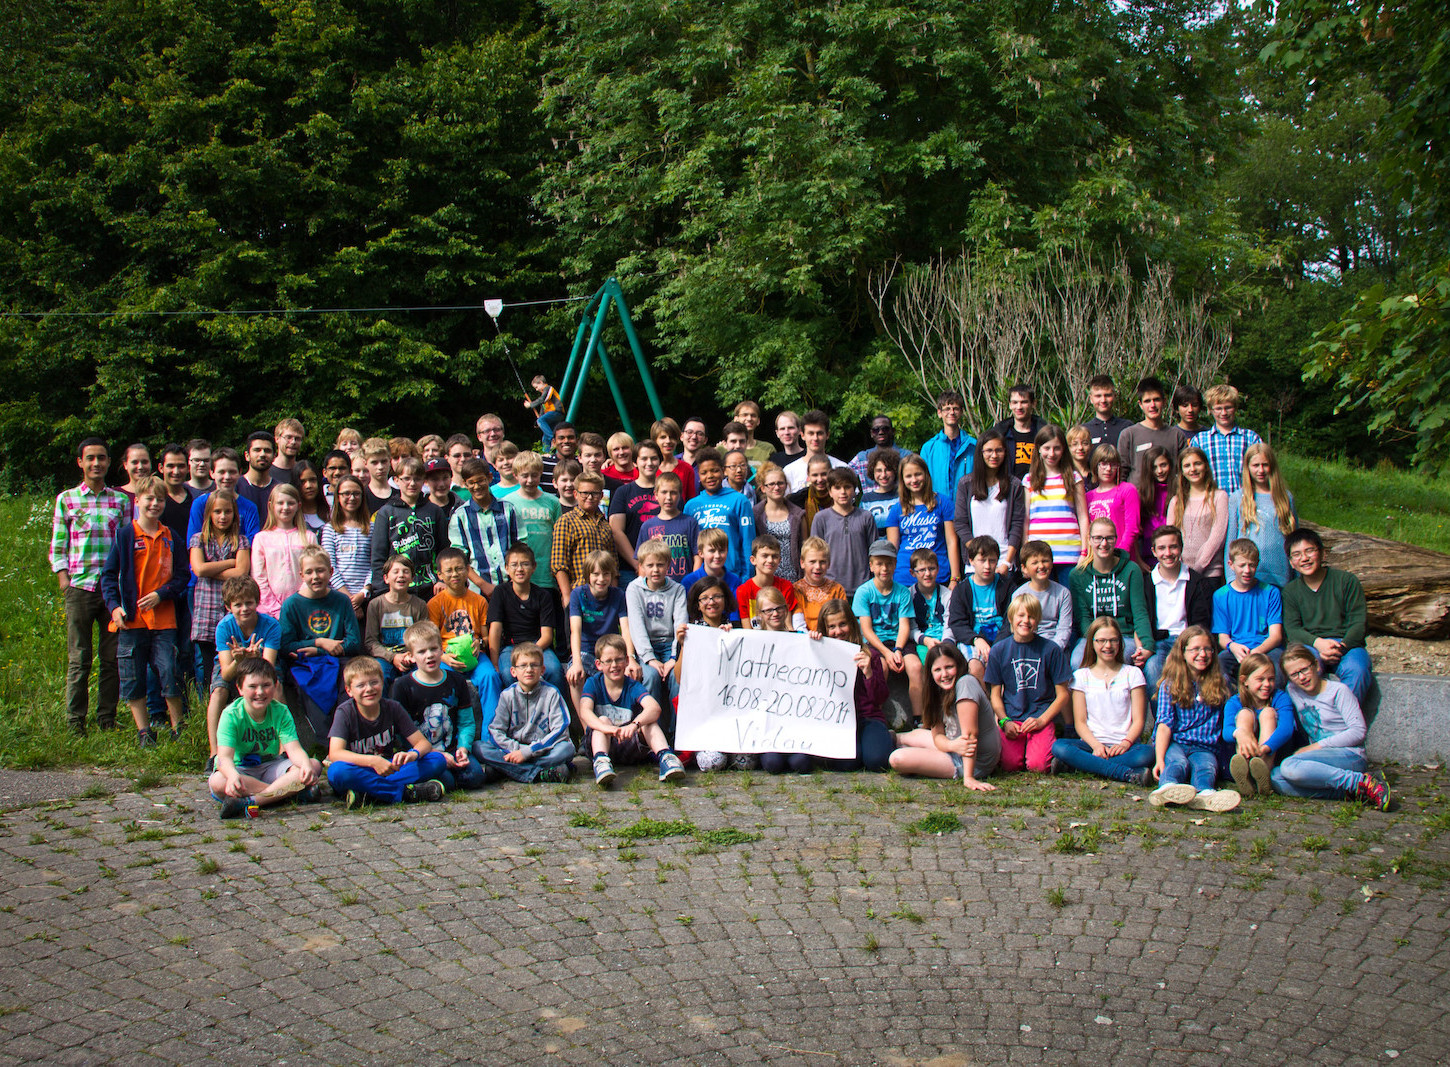
\includegraphics[width=0.85\textwidth]{mathecamp-gruppenfoto}
  \end{center}
\end{frame}

\section{Bildquellen}

\begin{frame}\frametitle{Bildquellen}
  \tiny
  \url{https://upload.wikimedia.org/wikipedia/commons/9/99/Vi_Hart.jpg}
  \url{http://joachim-reichel.org/software/fraktal/mandelbrot_large.png}
  \url{https://commons.wikimedia.org/wiki/File:Bellis_perennis_white_(aka).jpg}
  \url{http://www.maths.surrey.ac.uk/hosted-sites/R.Knott/Fibonacci/coneflower.jpg} (Tim Stone)
  \url{http://www.bibliotecapleyades.net/imagenes_ciencia2/conscious_universe472_02.jpg}
  \url{http://www.education.txstate.edu/ci/faculty/dickinson/PBI/PBIFall06/GeoNature/Content/Fibonacci_Lesson_files/image037.gif}
  \mbox{\url{http://www.sciencedump.com/sites/default/files/styles/article_width/public/field/gallery/8247962.jpg}}
  \par
\end{frame}

\backupend

\end{document}

Plan of the talk:

1. Images of spirals in nature; notice Fibonacci numbers.
2. Infinite continued fraction:
   * Example with [1; 2, ...]
   * More examples (only listed)
   * Euclidean algorithm (with illustration?)
   * Theorem about best approximation
3. Approximation of pi
   * List original sources for 22/7 and 355/113
   * Explain using continued fractions
4. Spirals in nature
   * angle, need "most irrational number"
   * golden ratio (also explain as a ratio)
   * simulations
5. Fibonacci numbers in the Mandelbrot fractal
6. Vi Hart

Mention rational tangles?

Relation to the number 5.


XXX: Mönchstory heraussuchen

* sqrt[12]{2}-Basis erwähnen
* Beginn der Mathematik thematisieren; so Verbindung zur Zahl 5 schaffen.
* https
